\documentclass{article}%
\usepackage[T1]{fontenc}%
\usepackage[utf8]{inputenc}%
\usepackage{lmodern}%
\usepackage{textcomp}%
\usepackage{lastpage}%
\usepackage{geometry}%
\geometry{tmargin=2cm,lmargin=2cm,rmargin=2cm,bmargin=2cm}%
\usepackage{graphicx}%
\usepackage{float}%
\usepackage{booktabs}%
\usepackage{rotating}%
%
\title{Relatório de Análise de Performance dos Modelos de Resposta}%
\date{\today}%
%
\begin{document}%
\normalsize%
\maketitle%
\section*{Introdução}%
\label{sec:Introduo}%
Este relatório apresenta uma análise completa dos modelos de resposta, avaliando a similaridade entre as respostas geradas e as respostas de referência. Foram calculadas diversas métricas de similaridade e realizadas análises estatísticas e visuais para identificar padrões de performance, inconsistências e possíveis pontos de melhoria. O objetivo é fornecer subsídios para interpretar os dados de forma objetiva, auxiliando na tomada de decisões para ajustes nos algoritmos.

%
\section*{Metodologia}%
\label{sec:Metodologia}%
A análise foi realizada em duas etapas principais:\newline%
\newline%
%
\begin{itemize}%
\item Carregamento dos dados: os dados foram extraídos de um arquivo pickle e convertidos para dicionários, possibilitando o acesso às respostas dos modelos e às respostas de referência.%
\item Processamento e análise: foram calculadas diversas métricas de similaridade, estatísticas descritivas e correlações. Além disso, foram gerados diversos gráficos (barras, histogramas, boxplots, heatmaps e scatter plots) para facilitar a interpretação visual dos resultados.%
\end{itemize}%
Cada gráfico ou tabela vem acompanhado de uma breve explicação sobre como interpretá{-}lo, de modo que o leitor possa compreender os pontos principais de cada análise.

%
\section*{Resultados}%
\label{sec:Resultados}%
\subsection*{Estatísticas de Similaridade Geral}%
\label{subsec:EstatsticasdeSimilaridadeGeral}%
Nesta seção são apresentadas as estatísticas descritivas da overall similarity dos modelos. Valores médios e medianos mais elevados indicam melhor aderência às respostas de referência, enquanto um alto desvio padrão pode indicar maior variabilidade.%
\newline%
Foram gerados os seguintes gráficos para visualizar esses dados:%


\begin{figure}[H]%
\centering%
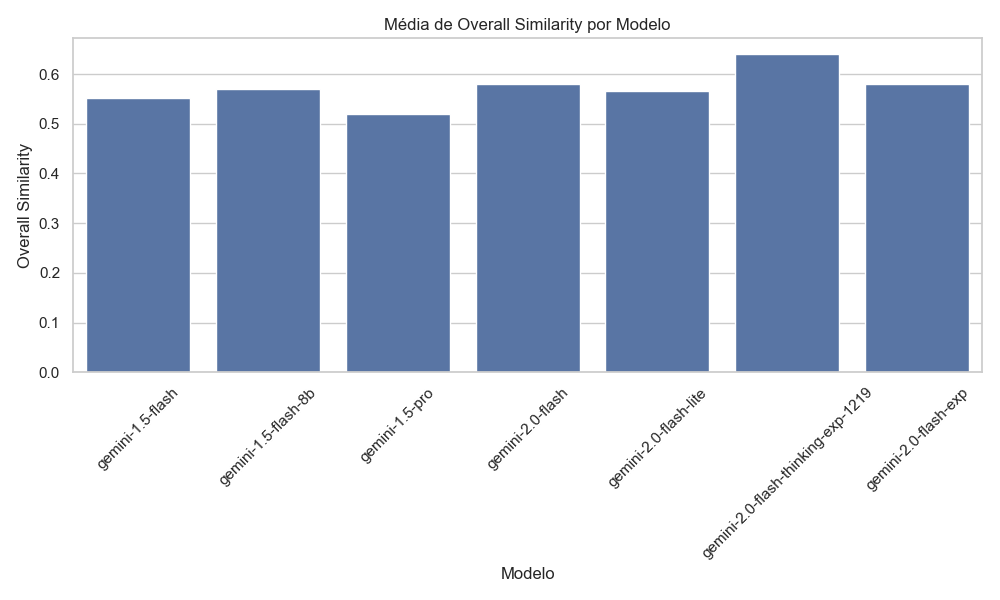
\includegraphics[width=0.8\textwidth]{analysis_results/barplot_overall_similarity.png}%
\caption{Gráfico de Barras – Média de Overall Similarity por Modelo. Observe as diferenças de desempenho entre os modelos.}%
\end{figure}

%


\begin{figure}[H]%
\centering%
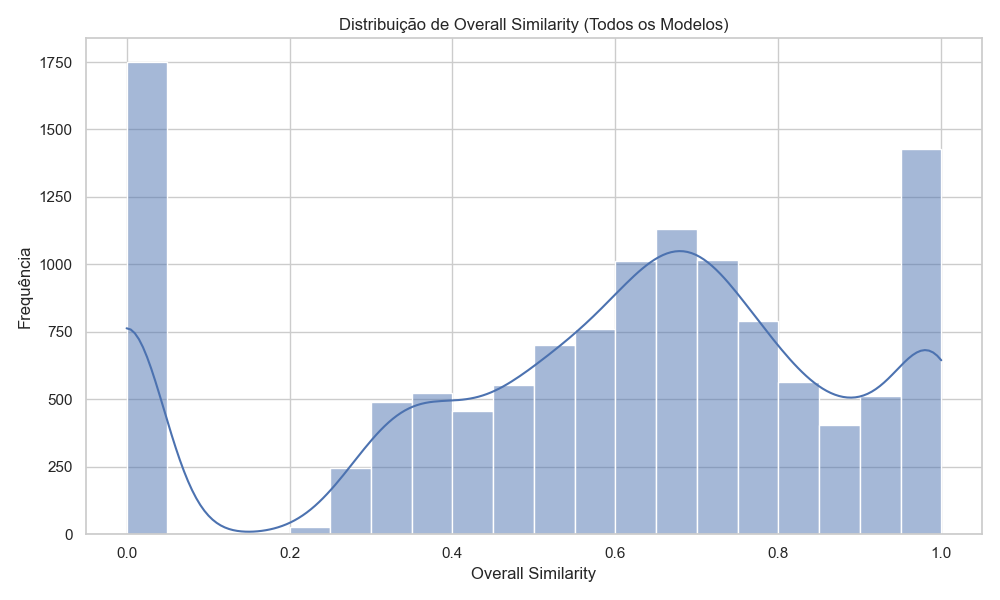
\includegraphics[width=0.8\textwidth]{analysis_results/histogram_overall_similarity.png}%
\caption{Histograma – Distribuição de Overall Similarity. Permite visualizar a dispersão dos valores obtidos.}%
\end{figure}

%


\begin{figure}[H]%
\centering%
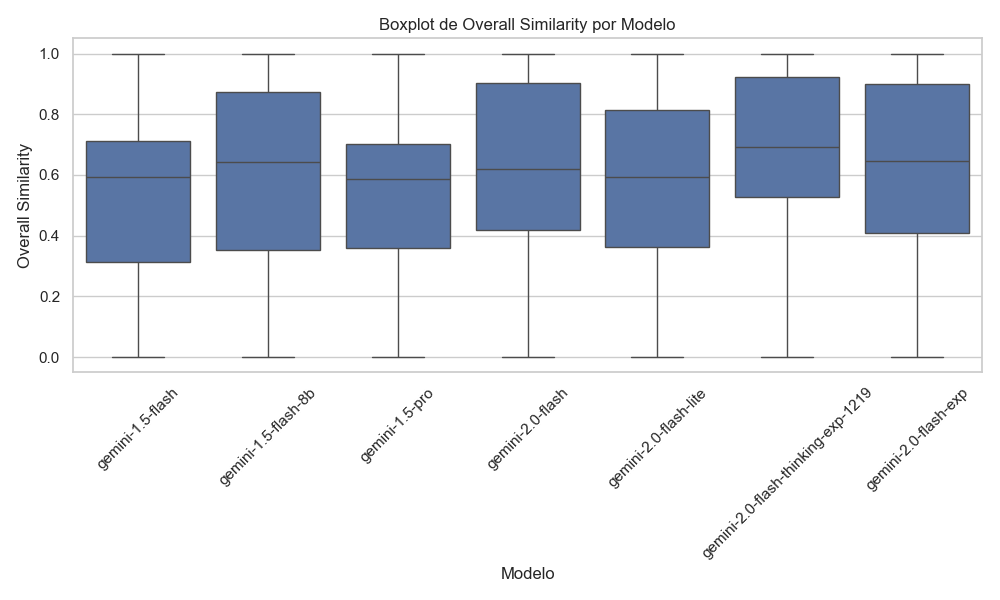
\includegraphics[width=0.8\textwidth]{analysis_results/boxplot_overall_similarity.png}%
\caption{Boxplot – Overall Similarity por Modelo. Facilita a identificação de mediana, quartis e outliers.}%
\end{figure}

%
\subsection*{Correlação entre Métricas de Similaridade}%
\label{subsec:CorrelaoentreMtricasdeSimilaridade}%
Nesta análise, avaliamos a correlação entre as diferentes métricas de similaridade (score keys). O heatmap abaixo mostra a força da correlação entre cada par de métricas: valores próximos de 1 ou {-}1 indicam forte correlação, enquanto valores próximos de 0 sugerem correlação fraca ou inexistente.%


\begin{figure}[H]%
\centering%
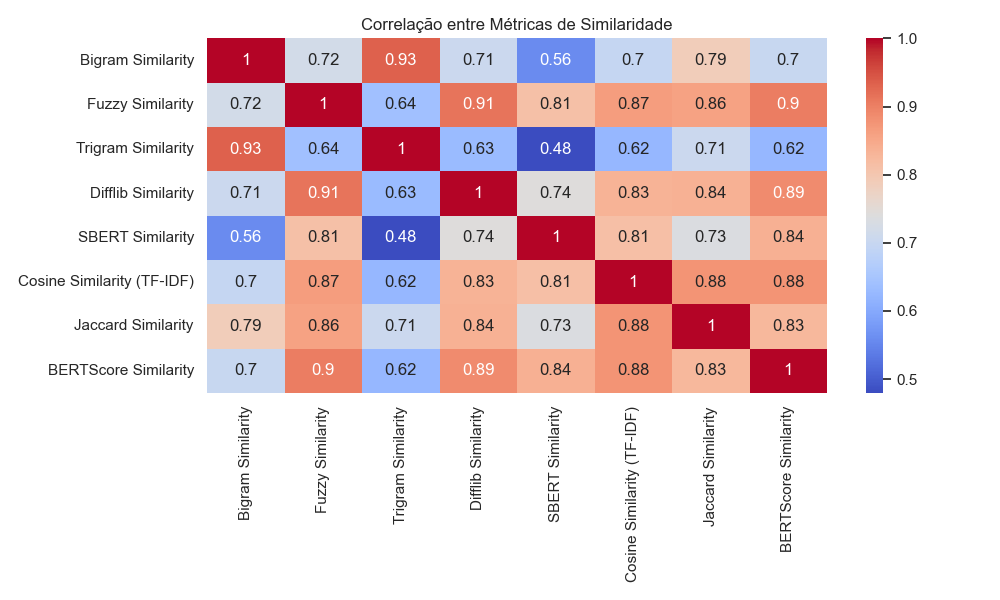
\includegraphics[width=0.8\textwidth]{analysis_results/heatmap_score_keys_correlation.png}%
\caption{Heatmap – Correlação entre as Métricas de Similaridade.}%
\end{figure}

%
\newline%
Além do heatmap, foram gerados scatter plots individuais comparando cada métrica com a overall similarity. Esses gráficos podem ser consultados nos anexos para análises mais detalhadas.

%
\subsection*{Correlação entre Overall Similarity e Média dos Scores}%
\label{subsec:CorrelaoentreOverallSimilarityeMdiadosScores}%
Esta seção apresenta a relação entre a overall similarity e a média dos scores detalhados (avg\textbackslash{}\_metric). O scatter plot a seguir permite identificar se existe uma tendência linear entre essas duas medidas, o que indicaria consistência na avaliação dos modelos.%


\begin{figure}[H]%
\centering%
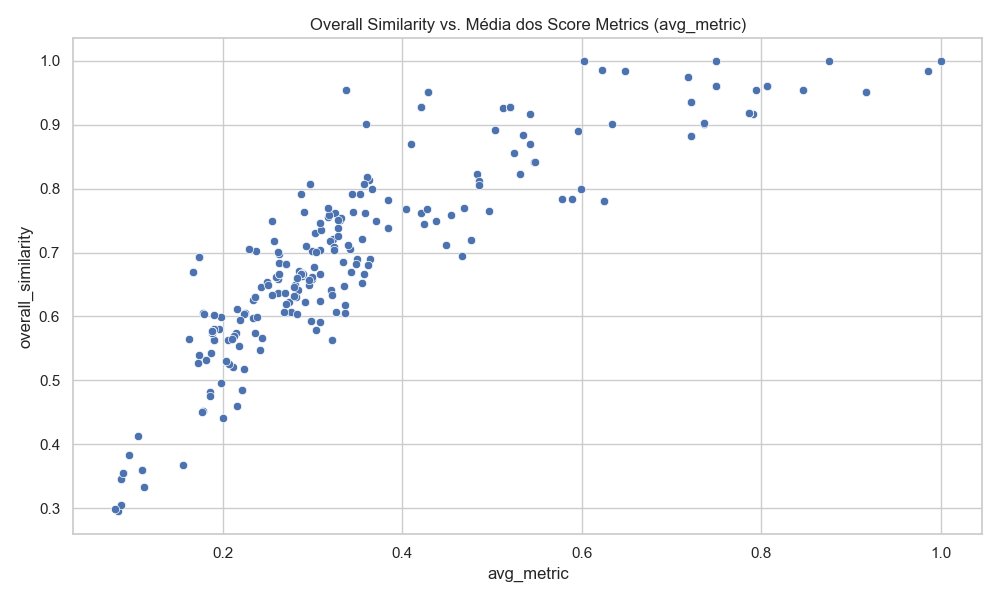
\includegraphics[width=0.8\textwidth]{analysis_results/scatter_overall_vs_avg_metric.png}%
\caption{Scatter Plot – Overall Similarity vs. Média dos Score Metrics (avg\textbackslash{}\_metric).}%
\end{figure}

%
\subsection*{Análise de Casos 'Unanswerable'}%
\label{subsec:AnlisedeCasosUnanswerable}%
Nesta parte, são analisados os casos em que os modelos não forneceram respostas (unanswerable). Os gráficos abaixo, apresentados lado a lado, mostram respectivamente a contagem desses casos e a relação entre a overall similarity e a condição de unanswerable. Em geral, uma baixa overall similarity pode estar associada a questões sem resposta.%


\begin{figure}[H]%
\begin{minipage}[b]{0.45\textwidth}%
\centering%
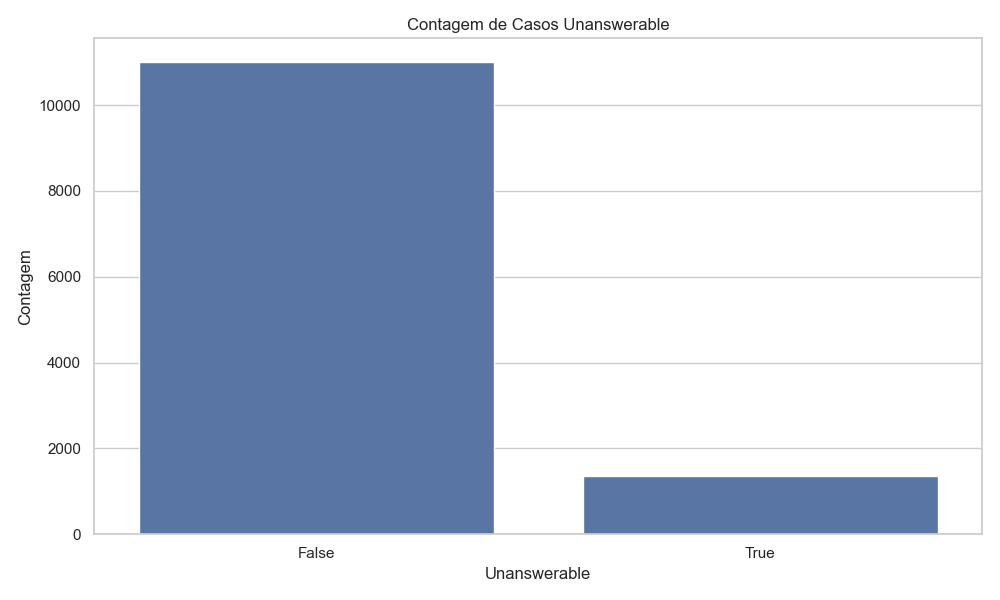
\includegraphics[width=\linewidth]{analysis_results/count_unanswerable.png}%
\caption*{Contagem de Casos Unanswerable.}%
\end{minipage}\hfill%
\begin{minipage}[b]{0.45\textwidth}%
\centering%
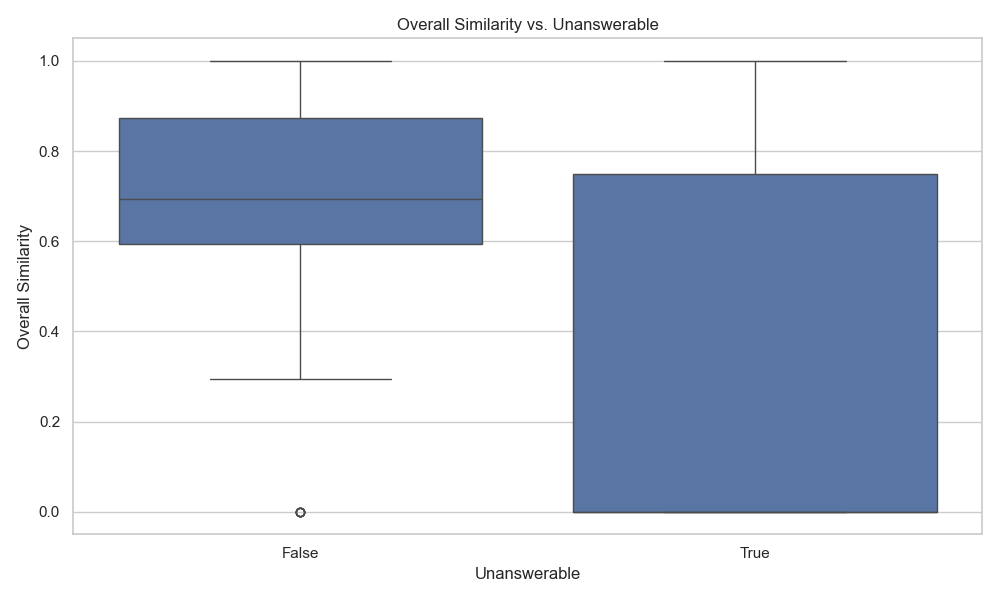
\includegraphics[width=\linewidth]{analysis_results/boxplot_overall_vs_unanswerable.png}%
\caption*{Boxplot – Overall Similarity vs. Unanswerable.}%
\end{minipage}%
\end{figure}

%
\subsection*{Correlação Inter{-}Modelos}%
\label{subsec:CorrelaoInter{-}Modelos}%
Esta análise verifica a correlação da overall similarity entre os diferentes modelos. Utilizando uma pivot table, foi calculada a correlação entre os modelos, cuja visualização por meio de um heatmap facilita a identificação de similaridades ou discrepâncias na performance entre eles.%


\begin{figure}[H]%
\centering%
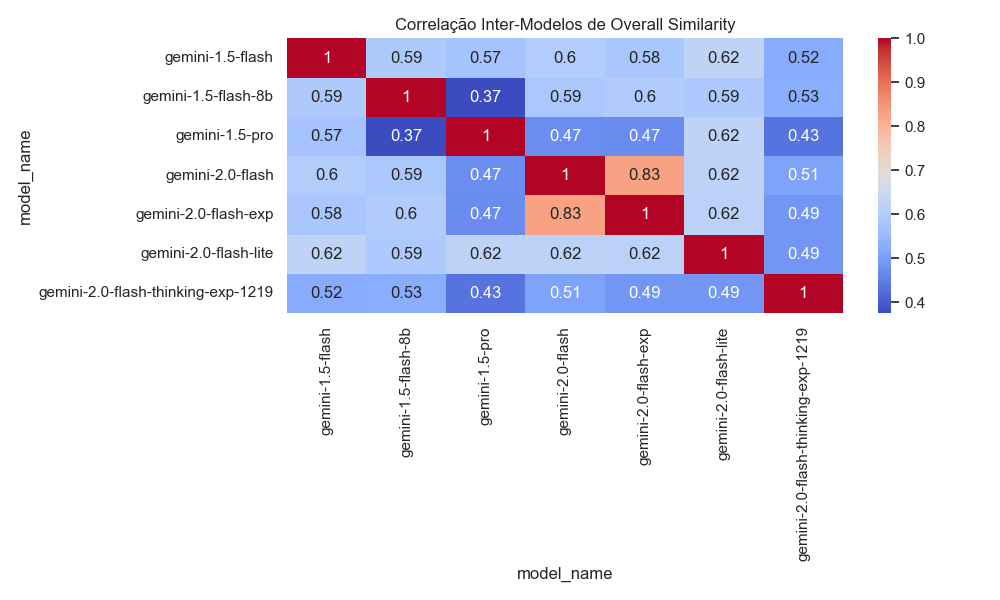
\includegraphics[width=0.8\textwidth]{analysis_results/heatmap_inter_model_corr.png}%
\caption{Heatmap – Correlação Inter{-}Modelos de Overall Similarity.}%
\end{figure}

%
\subsection*{Estatísticas Agregadas das Métricas Detalhadas}%
\label{subsec:EstatsticasAgregadasdasMtricasDetalhadas}%
A seguir, serão apresentadas diversas tabelas, cada uma correspondendo a um score específico. Em cada tabela, estão exibidas as estatísticas agregadas – média, mediana, desvio padrão, valor mínimo e valor máximo – agrupadas por modelo. Essas métricas auxiliam na identificação de padrões e na avaliação da consistência dos scores obtidos.%
\subsubsection*{Estatísticas para o Score: aggregated\_BERTScore Similarity}%
\begin{table}[H]%
\centering%
\begin{tabular}{llllll}
\toprule
 & mean & median & std & min & max \\
model_name &  &  &  &  &  \\
\midrule
gemini-1.5-flash & 0.6944 & 0.6875 & 0.0989 & 0.5143 & 1.0000 \\
gemini-1.5-flash-8b & 0.7423 & 0.7183 & 0.1223 & 0.4514 & 1.0000 \\
gemini-1.5-pro & 0.6761 & 0.6737 & 0.0856 & 0.4920 & 1.0000 \\
gemini-2.0-flash & 0.7567 & 0.7350 & 0.1212 & 0.4514 & 1.0000 \\
gemini-2.0-flash-exp & 0.7570 & 0.7410 & 0.1212 & 0.5236 & 1.0000 \\
gemini-2.0-flash-lite & 0.7303 & 0.7075 & 0.1186 & 0.4905 & 1.0000 \\
gemini-2.0-flash-thinking-exp-1219 & 0.7597 & 0.7412 & 0.1171 & 0.5076 & 1.0000 \\
\bottomrule
\end{tabular}
%
\end{table}%
\vspace{0.5cm}%
\subsubsection*{Estatísticas para o Score: aggregated\_Bigram Similarity}%
\begin{table}[H]%
\centering%
\begin{tabular}{llllll}
\toprule
 & mean & median & std & min & max \\
model_name &  &  &  &  &  \\
\midrule
gemini-1.5-flash & 0.0755 & 0.0204 & 0.1526 & 0.0000 & 1.0000 \\
gemini-1.5-flash-8b & 0.1319 & 0.0105 & 0.2497 & 0.0000 & 1.0000 \\
gemini-1.5-pro & 0.0567 & 0.0157 & 0.1109 & 0.0000 & 1.0000 \\
gemini-2.0-flash & 0.1667 & 0.0143 & 0.2774 & 0.0000 & 1.0000 \\
gemini-2.0-flash-exp & 0.1690 & 0.0185 & 0.2748 & 0.0000 & 1.0000 \\
gemini-2.0-flash-lite & 0.1323 & 0.0101 & 0.2376 & 0.0000 & 1.0000 \\
gemini-2.0-flash-thinking-exp-1219 & 0.1306 & 0.0000 & 0.2516 & 0.0000 & 1.0000 \\
\bottomrule
\end{tabular}
%
\end{table}%
\vspace{0.5cm}%
\subsubsection*{Estatísticas para o Score: aggregated\_Cosine Similarity (TF-IDF)}%
\begin{table}[H]%
\centering%
\begin{tabular}{llllll}
\toprule
 & mean & median & std & min & max \\
model_name &  &  &  &  &  \\
\midrule
gemini-1.5-flash & 0.2831 & 0.2308 & 0.2346 & 0.0000 & 1.0000 \\
gemini-1.5-flash-8b & 0.3795 & 0.2912 & 0.3335 & 0.0000 & 1.0000 \\
gemini-1.5-pro & 0.2521 & 0.2152 & 0.1995 & 0.0000 & 1.0000 \\
gemini-2.0-flash & 0.3915 & 0.2925 & 0.3330 & 0.0000 & 1.0000 \\
gemini-2.0-flash-exp & 0.3952 & 0.3112 & 0.3295 & 0.0000 & 1.0000 \\
gemini-2.0-flash-lite & 0.3337 & 0.2416 & 0.3057 & 0.0000 & 1.0000 \\
gemini-2.0-flash-thinking-exp-1219 & 0.4041 & 0.3179 & 0.3461 & 0.0000 & 1.0000 \\
\bottomrule
\end{tabular}
%
\end{table}%
\vspace{0.5cm}%
\subsubsection*{Estatísticas para o Score: aggregated\_Difflib Similarity}%
\begin{table}[H]%
\centering%
\begin{tabular}{llllll}
\toprule
 & mean & median & std & min & max \\
model_name &  &  &  &  &  \\
\midrule
gemini-1.5-flash & 0.2287 & 0.1615 & 0.2324 & 0.0000 & 1.0000 \\
gemini-1.5-flash-8b & 0.3540 & 0.2562 & 0.3134 & 0.0000 & 1.0000 \\
gemini-1.5-pro & 0.1889 & 0.1386 & 0.1894 & 0.0000 & 1.0000 \\
gemini-2.0-flash & 0.4001 & 0.3125 & 0.3162 & 0.0000 & 1.0000 \\
gemini-2.0-flash-exp & 0.4055 & 0.3320 & 0.3152 & 0.0000 & 1.0000 \\
gemini-2.0-flash-lite & 0.3371 & 0.2516 & 0.2969 & 0.0000 & 1.0000 \\
gemini-2.0-flash-thinking-exp-1219 & 0.3888 & 0.3016 & 0.3078 & 0.0000 & 1.0000 \\
\bottomrule
\end{tabular}
%
\end{table}%
\vspace{0.5cm}%
\subsubsection*{Estatísticas para o Score: aggregated\_Fuzzy Similarity}%
\begin{table}[H]%
\centering%
\begin{tabular}{llllll}
\toprule
 & mean & median & std & min & max \\
model_name &  &  &  &  &  \\
\midrule
gemini-1.5-flash & 0.2894 & 0.2500 & 0.2340 & 0.0000 & 1.0000 \\
gemini-1.5-flash-8b & 0.4147 & 0.3700 & 0.2912 & 0.0000 & 1.0000 \\
gemini-1.5-pro & 0.2505 & 0.2200 & 0.2013 & 0.0000 & 1.0000 \\
gemini-2.0-flash & 0.4613 & 0.4000 & 0.2900 & 0.0000 & 1.0000 \\
gemini-2.0-flash-exp & 0.4664 & 0.4200 & 0.2883 & 0.0000 & 1.0000 \\
gemini-2.0-flash-lite & 0.3968 & 0.3600 & 0.2800 & 0.0000 & 1.0000 \\
gemini-2.0-flash-thinking-exp-1219 & 0.4470 & 0.4100 & 0.2829 & 0.0000 & 1.0000 \\
\bottomrule
\end{tabular}
%
\end{table}%
\vspace{0.5cm}%
\subsubsection*{Estatísticas para o Score: aggregated\_Jaccard Similarity}%
\begin{table}[H]%
\centering%
\begin{tabular}{llllll}
\toprule
 & mean & median & std & min & max \\
model_name &  &  &  &  &  \\
\midrule
gemini-1.5-flash & 0.1728 & 0.1136 & 0.2034 & 0.0000 & 1.0000 \\
gemini-1.5-flash-8b & 0.2857 & 0.1500 & 0.3259 & 0.0000 & 1.0000 \\
gemini-1.5-pro & 0.1413 & 0.1014 & 0.1575 & 0.0000 & 1.0000 \\
gemini-2.0-flash & 0.3089 & 0.1667 & 0.3242 & 0.0000 & 1.0000 \\
gemini-2.0-flash-exp & 0.3119 & 0.1818 & 0.3204 & 0.0000 & 1.0000 \\
gemini-2.0-flash-lite & 0.2506 & 0.1429 & 0.2831 & 0.0000 & 1.0000 \\
gemini-2.0-flash-thinking-exp-1219 & 0.3032 & 0.1779 & 0.3327 & 0.0000 & 1.0000 \\
\bottomrule
\end{tabular}
%
\end{table}%
\vspace{0.5cm}%
\subsubsection*{Estatísticas para o Score: aggregated\_SBERT Similarity}%
\begin{table}[H]%
\centering%
\begin{tabular}{llllll}
\toprule
 & mean & median & std & min & max \\
model_name &  &  &  &  &  \\
\midrule
gemini-1.5-flash & 0.5127 & 0.5569 & 0.2606 & -0.0906 & 1.0000 \\
gemini-1.5-flash-8b & 0.5942 & 0.6126 & 0.2885 & -0.1126 & 1.0000 \\
gemini-1.5-pro & 0.4844 & 0.5332 & 0.2473 & -0.1219 & 1.0000 \\
gemini-2.0-flash & 0.5903 & 0.6042 & 0.2880 & -0.0952 & 1.0000 \\
gemini-2.0-flash-exp & 0.5907 & 0.6066 & 0.2871 & -0.1078 & 1.0000 \\
gemini-2.0-flash-lite & 0.5320 & 0.5592 & 0.2940 & -0.1126 & 1.0000 \\
gemini-2.0-flash-thinking-exp-1219 & 0.6212 & 0.6387 & 0.2834 & -0.1126 & 1.0000 \\
\bottomrule
\end{tabular}
%
\end{table}%
\vspace{0.5cm}%
\subsubsection*{Estatísticas para o Score: aggregated\_Trigram Similarity}%
\begin{table}[H]%
\centering%
\begin{tabular}{llllll}
\toprule
 & mean & median & std & min & max \\
model_name &  &  &  &  &  \\
\midrule
gemini-1.5-flash & 0.0492 & 0.0000 & 0.1374 & 0.0000 & 1.0000 \\
gemini-1.5-flash-8b & 0.0938 & 0.0000 & 0.2235 & 0.0000 & 1.0000 \\
gemini-1.5-pro & 0.0322 & 0.0000 & 0.0912 & 0.0000 & 1.0000 \\
gemini-2.0-flash & 0.1244 & 0.0000 & 0.2549 & 0.0000 & 1.0000 \\
gemini-2.0-flash-exp & 0.1253 & 0.0000 & 0.2519 & 0.0000 & 1.0000 \\
gemini-2.0-flash-lite & 0.0948 & 0.0000 & 0.2134 & 0.0000 & 1.0000 \\
gemini-2.0-flash-thinking-exp-1219 & 0.0855 & 0.0000 & 0.2152 & 0.0000 & 1.0000 \\
\bottomrule
\end{tabular}
%
\end{table}%
\vspace{0.5cm}

%
\section*{Discussão}%
\label{sec:Discusso}%

A análise dos dados indica que o modelo \textbf{gemini-2.0-flash-thinking-exp-1219} apresentou a maior média de overall similarity (0.64), 
enquanto o modelo \textbf{gemini-1.5-pro} apresentou a menor média (0.52). Essa diferença ressalta variações na performance 
dos modelos em aderência às respostas de referência.

Adicionalmente, observa-se que o percentual de casos com dicionário de scores vazio foi mais elevado para o modelo 
\textbf{gemini-1.5-flash-8b} (23.92%), sugerindo que podem haver dificuldades na geração ou na coleta dos scores para esse modelo.

A análise das estatísticas agregadas das métricas detalhadas evidencia variações na consistência dos modelos, o que pode ser explorado 
para identificar possíveis ajustes nos algoritmos de resposta.

%
\section*{Anexos}%
\label{sec:Anexos}%
Os anexos deste relatório reúnem os arquivos CSV gerados e todos os gráficos produzidos durante a análise, tais como:%
\begin{itemize}%
\item overall\_stats.csv%
\item empty\_scores\_frequency.csv%
\item variation\_data.csv%
\item aggregated\_metrics.csv%
\item overall\_similarity.csv%
\item detailed\_similarity.csv%
\end{itemize}%
Além disso, todos os gráficos (barplots, histogramas, boxplots, heatmaps e scatter plots) podem ser conferidos na pasta 'analysis\_results'.

%
\section*{Referências}%
\label{sec:Referncias}%
As principais bibliotecas e ferramentas utilizadas para a geração deste relatório foram:%
\begin{itemize}%
\item \textbf{pandas} e \textbf{numpy} para manipulação e análise dos dados.%
\item \textbf{matplotlib} e \textbf{seaborn} para a criação dos gráficos.%
\item \textbf{PyLaTeX} para a montagem do documento LaTeX.%
\end{itemize}

%
\end{document}